\chapter{Određivanje sličnosti izvornih kodova}

Ne postoji sustav specijaliziran za detekciju plagijata koji može sa sto postotnom sigurnošću utvrditi da je nešto plagijat. Kako bi odredili plagijat potreban je ljudski faktor.  Odmah možemo uočiti da to nije baš uvijek efikasno, kada bi morali pronaći plagijate među tisućama dokumenata čovjeku bi trebalo puno vremena. Upravo iz tog razloga razvijamo sustav koji bi odredio sličnost među parovima dokumenata te izbacio parove za koje smatra da nikako ne mogu biti plagijat te uvelike ubrzao i olakšao posao ljudima. Dokumenti mogu biti teksutalne datoteke, izvorni kodovi, pjesme, itd. \\
	
	Određivanje sličnosti izvornih kodova u svrhu detekcije plagijata je relativno neistraženo područje. Postoje dva vrlo slična, ali sada već stara sustava (nastali su prije više od 10 godina op.a)  \cite{moss} \cite{jplag} koji se baziraju na računanju otiska(eng.~$document fingerprint$) izvornog koda algoritmom $winnowing$ koji je detaljnije opisan u \cite{winnowing}. $Turtle$, kao i sustav implementiran na završnom radu \cite{plagijator}, koristi $winnowing$ za račun otiska izvornog koda te preoblikovanje izvornog koda prije nego se otisak računa(detaljnije opisano u radu \cite{dorian}), no s dodatnim poboljšanjima. Neka od poboljšanja su veći broj preoblikovanja, što rezultira u boljim mjerama sličnosti i brže ukupno vrijeme. U nastavku poglavlja detaljnije su opisani koraci kojim sustav dolazi do mjera sličnosti, najvažnije pomoćne strukture podataka i algoritmi te usporedba s performansama starog sustava.

\newpage
\newgeometry{bottom=25mm, top=25mm, right=25mm, left=30mm}

\section{Izračun otiska izvornog koda}

Otisak izvornog koda definiran je kao jedan podskup iz skupa izračunatih sažetaka(eng.~\textit{hash}) k-grama \cite{winnowing}. K-gram je uzastopni podniz duljine $k$. Odmah primjećujemo da k-grama ima $n-k-1$ za znakovni niz duljine $n$ te su ta dva broja vrlo blizu za manje vrijednosti $k$. Iako nigdje u literaturu nije navedeno koliko točno bi trebao biti $k$, najbolje rezultate su pokazale manje vrijednosti(otprilike prosjek duljine prosječnih duljina ključnih riječi programskog jezika na kojem se radi).  Iz tog razloga potreban nam je efikasan algoritam kako bi izračunali sažetke svakog k-grama. Jedan od takvih algoritama je \textit{Rabin-Karp} \cite{rabin-karp}.

\subsection{Rabin-Karp algoritam}

\textit{Rabin-Karp} je algoritam koji nam u linearnoj $O(n)$ složenosti računa sažetke svih k-grama ulaznog znakovnog niza. Algoritam radi tako da postupno gradi rješenje, iz $i^{tog}$ sažetka se računa $i+1$. Ako k-gram zapišemo kao $c_1...c_k$ tada sažetak računamo:

\begin{equation}
	H(c_1...c_k) = c_1 * b^{k-1} + c_1 * b^{k-2} + ... + c_k
\end{equation}

\noindent gdje su $b$ baza, a $c_i$ ascii vrijednost $i^{tog}$ znaka. Za bazu se uzima prost broj kako bi se izbjegle kolizije.

\noindent Idući sažetak tada računamo tako da prethodno izračunatom sažetku oduzmemo prvi član, pomnožimo sve s $b$ i dodamo novi znak:
	
\begin{equation}
	H(c_2...c_k+1) = (H(c_1...c_k) - c_1 * b^{k-1}) * b + c_{k+1}
\end{equation}

\noindent Svaki uzastopni sažetak izračunat je uz samo tri operacije i tu možemo shvatiti linearnu složenost algoritma. Bitno je naglasiti da se iz ulaznog znakovnog niza prije računanja izbacuju nebitni znakovni poput razmaka.
\newpage

\subsection{Winnowing}

\textit{Winnowing} je algoritam za računanje otiska izvornog koda. Na ulaz prima niz sažetaka ranije izračunatih \textit{Rabin-Karp} algoritmom te ispisuje izračunati otisak. U nastavku je pseudokod algoritma:

\begin{algorithm}
\caption{Winnowing}

\begin{algorithmic}
\STATE{\textbf{Ulaz:} $K$ -- niz sažetaka k-grama.}
\STATE{\textbf{Izlaz:} otisak $F$.}
\STATE{windows := split\_to\_windows(w)}
\FOR{($i := 0; i < n; ++i$)}
	\STATE{w\_min := min(windows[i])}
	\IF{(more\_than\_one\_same\_val)}
		\IF{(w\_min is rightmost)}
			\STATE{F.append(w\_min)}
		\ENDIF
	\ENDIF
\ENDFOR
\RETURN{F}

\end{algorithmic}
\end{algorithm}

\noindent Primjer rada \textit{Rabin-Karp} i \textit{Winnowing} algoritama vidimo na slici \ref{fig:winnowing}.

\begin{figure}[htb]
	\centering
	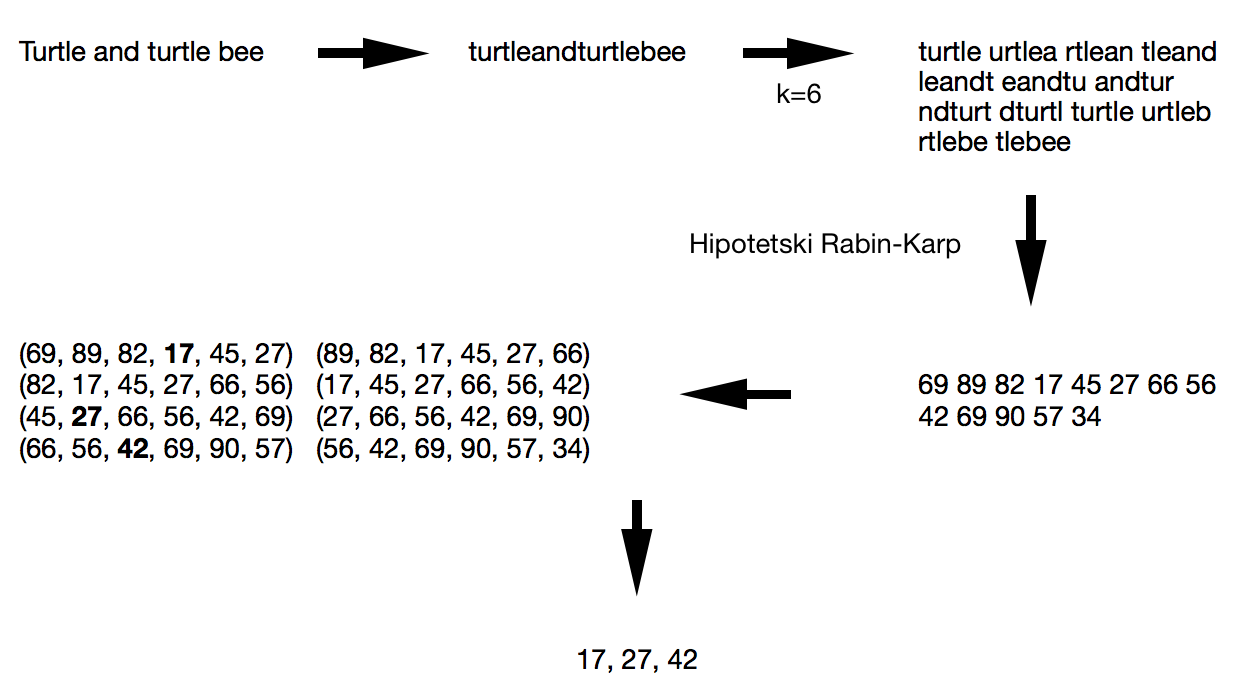
\includegraphics[width=0.8\textwidth, height=7cm, keepaspectratio]{fig/winnowing.png}
	\caption{Primjer rada algoritma $winnowing$}
	\label{fig:winnowing}
\end{figure}


\section{Preoblikovanje izvornog koda}

Glavni razlog za korištenje preoblikovanja koda prije nego krenemo računati otisak je taj što algoritmi za računanje otiska pa tako i $winnowing$ nisu otporni na mnoge pokušaje izmjene koda kako ih se ne bi detektiralo kao plagijate. Nabrojimo neke od njih:

	\begin{itemize}
		\item Dodavanje beskorisnih komentara
		\item Dodavanje beskorisnog koda
		\item Dodavanje praznina
		\item Zamjena imena varijabli
		\item Promjena jedne petlje u drugu
		\item Rastav naredbi na podbaredbe
		\item Izdvajanje koda u funkcije
		\item Promjena redoslijeda naredbi
	\end{itemize}
	
\noindent Odmah možemo primjetiti da je $winnowing$ otporan na dodavanje praznina jer se one brišu prije računanja sažetaka. Također izdvajanje koda u funkcije se detektira jer nema razlike gdje točno se isječci koda nalaze za rezultat algoritma. Za ostale modifikacije trebamo napisati posebne funkcije koje će preoblikovati izvorni kod kako bi i one mogle biti detektirane. Naravno, modifikacije kao što je rastav naredbi na podnaredbe  je jako teško detektirati bez korištenja jezičnog prevodica i neke vrste sintaksnih stabala te se tu limitiramo i njih $Turtle$ ne zna detektirati. U nastavku poglavlja opisana su korištena preoblikovanja izvornog koda. Treba naglasiti da ovakvih preoblikovanja može biti jako puno te je sustav dizajniran tako da se svako preoblikovanje može vrlo lako dodati.


\subsection{Zamjena imena varijabli}

Ideja je da se sva imena varijabli zamjene univerzalnim imenom, u ovom slučaju odabrano je ime \textit{var}. Također mijenjamo i sve konstante kako bi mogli detektirati i promjenu redoslijeda naredbi. Prvo sve te varijable moramo pronaći unutar izvornog koda, a to radimo tako da izgradimo automat za željeni programski jezik koji će nam znati reći kada smo u stanju imena varijable. Kako bi automat znao razlikovati ključnu riječ od varijable potrebno je izgraditi strukturu podataka koja će mu reći promatra li ključnu riječ jezika. Za te potrebe izgrađeno je prefiksno stablo \cite{prefix-tree} od svih ključnih riječi koje nam tu funkcionalnost omogućava u jako brzom vremenu, zbog male duljine ključnih riječi možemo reći u $O(1)$. Implementirani automat također prepoznaje stanje komentar te izbacuje sve komentare iz izvornog koda pa time rješavamo i modifikaciju dodavanjem komentara. U dodatku B \ref{before:after} vidimo izgled izvornog koda prije i poslije izvršavanja automata. \newline


\subsection{Zamjena while petlji u for petlje}

Ovdje je opisan postupak za programski jezik $C++$, no postupak se može uz male preinake primjeniti i na sve poznatije programske jezike. Prvo primjetimo oblik $while$ petlje:
\begin{lstlisting}
	init; while(test){ body; post; }
\end{lstlisting}

\noindent te ga zapišimo kao $for$ petlju:
\begin{lstlisting}
	for(init; test; post){ body; }
\end{lstlisting}

\noindent Sada samo pronađemo ovakve isječke unutar koda i zamijenimo ih, npr. korištenjem regeks operacija.

\section{Izračun sličnosti izvornih kodova}

Nakon što smo izračunali otisak izvornog koda još samo trebamo izračunati sličnosti svih parova. Najprije se izračuna mapa indeksa(eng.~\textit{index mapping}) koja za svaki otisak sprema sve izvorne kodove u kojem se on nalazi. Nakon toga računaju se dvije sličnosti, sličnost prvog koda prema drugom kodu $x_{12}$ te sličnost drugog koda prema prvom kodu $x_{21}$ i to tako da se prebroje pojavljivanja otisaka koji su im zajednički te se taj broj normalizira ukupnim brojem otisaka prvog člana para. Dvije sličnosti imamo kako bi što bolje opisali slučajeve kada imamo dva izvorna koda koja imaju veliku razliku u broju linija. S ovakvim računanjem sličnosti također rješavamo problem dodavanja beskorisnog koda prethodno opisanog.  Za kraj nam samo ostaje definirati funkciju koja bi ove dvije sličnosti transformirala u jednu kako bi parove mogli sortirane prikazati u web aplikaciji:

\begin{equation}
	f(x_{12}, x_{21}) = (x_{12} + x_{21}) * min(x_{12}, x_{21})
\end{equation}

\noindent Odabrana je ova funkcija jer se u praksi pokazala kao odličan izbor. Ova funkcija nam također filtrira parove kako ne bi korisniku prikazivali parove koji sigurno nisu plagijati. 

\section{Usporedba sa starim sustavom}

Kao što je spomenuto ranije ovaj sustav je novo implementirana verzija sustava implementiranog za završni rad te su u ovom poglavlju uspoređeni ti sustavi. Najveća prednost novog sustava je u njegovoj brzini što vidimo na slici \ref{fig:execution_time}.

\begin{figure}[htb]
	\centering
	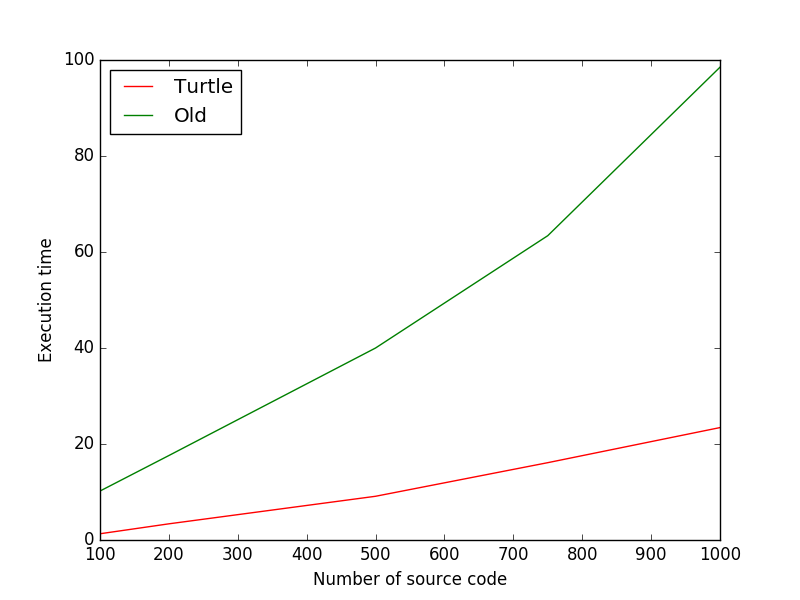
\includegraphics[width=0.9\textwidth,keepaspectratio]{fig/execution_time.png}
	\caption{Usporedba vremena izvršavanja}
	\label{fig:execution_time}
\end{figure}

\noindent Mjereno je vrijeme od primitka izvornih kodova pa sve do ispisa parova sličnosti. Možemo primjetiti da oba sustava imaju linearnu složenost, no zbog puno bolje i pametnije implementacije $Turtle$ je daleko bolji. $Turtle$ također zbog više preoblikovanja izvornog koda nudi bolju detekciju nekih modifikacija(npr. zamjena $for$ u $while$ petlje). Ostatak modifikacija te izračunatih sličnosti nisu posebno opisivani jer su vrlo slični već opisanima u \cite{plagijator}.
